\chapter{Ausgewählte Technologien}

\section{Git und GitLab}

\subsection{Versionskontrollsystem}
Oftmals arbeitet ein Entwickler oder ein Entwicklerteam an einem Softwareprojekt, um entweder Fehler zu beheben oder neue Funktionalitäten hinzuzufügen. Hierbei werden Änderungen am Quellcode durchgeführt, die regelmäßig gesichert werden müssen. Diese Änderungen können in manchen Fällen auch dazu führen, dass etwas anderes im Code nicht mehr so funktioniert wie es sollte. Dann werden weitere Änderungen gemacht, um wieder einen lauffähigen Stand herzustellen, jedoch kann es passieren, dass plötzlich gar nichts mehr funktioniert.

\mbox{}\\Abhilfe für dieses Problem bietet ein Versionskontrollsystem, auch als VCS (Version Control System) bezeichnet, das Änderungen in der Projektentwicklung festhält (Dirk 2019, vgl. \cite{vcs_2019}, 15.11.2020). Dadurch ist es möglich zu einem späteren beliebigen Zeitpunkt auf ältere Versionen des Systems zurückzugreifen, den aktuellen Code mit früheren Versionen zu vergleichen oder Bugfixes zu implementieren. Arbeiten mehrere Entwickler an denselben Dateien im Quellcode, so kann mitverfolgt werden, welche Person welche Änderungen gemacht hat. Ein Projekt, das mit einem VCS verwaltet wird, wird Repository genannt. Ein Repository kann als eine Art Datenbank mit allen Änderungen betrachtet werden, die die History repräsentieren. Diese Änderungen sind ein markierter Stand, ein sogenannter Commit, in der Projektentwicklung und werden als Working Copy gespeichert, die einer Kopie des gesamten Projektes entspricht. Ein Commit kann als Schnappschuss oder als kleiner Meilenstein betrachtet werden. Er beinhaltet neben der Working Copy einen Zeitstempel und eine Nachricht, die aussagt, was sich seit dem letzten Commit geändert hat. Die Entwicklungsarbeiten können dabei in mehreren Entwicklungszweigen (engl. Branches) erfolgen. Eine Abspaltung eines Projektes wird hingegen als Fork bezeichnet.

\newpage
Es gibt drei Arten von Version Control Systems:

\begin{itemize}
	\item \textbf{Lokal:} Lokale Versionskontrollsysteme funktionieren nur auf einem Rechner und versionieren eine einzige Datei. Insbesondere in Büroanwendungen kommen Tools wie Revision Control System (RCS) oder Source Code Control System (SCCS) zum Einsatz. Das Dokument speichert  dabei jede Version in seiner eigenen Datei.
	
	\begin{figure}[H]
	\begin{center}
		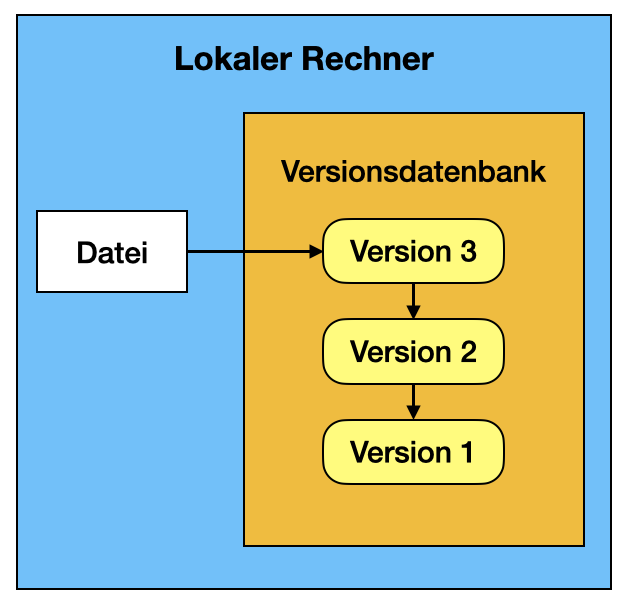
\includegraphics[scale=.65]{images/local_vcs.png}
	\end{center}
		\caption{Lokales Versionskontrollsystem}
	\end{figure}
	
	\item \textbf{Zentral:} Bei einem zentralisierten Versionskontrollsystem gibt es ein Respository, das sich mehrere 		Entwickler in einem Netzwerk miteinander teilen. Es handelt sich hierbei um ein Client-Server-System, das 		von zahlreichen kommerziellen Anbietern verwendet wird. Durch das Concurrent Versions System (CVS) 			wurde dieses Konzept berühmt, aber durch Subversion (SVN) neu implementiert.
	
	\begin{figure}[H]
	\begin{center}
		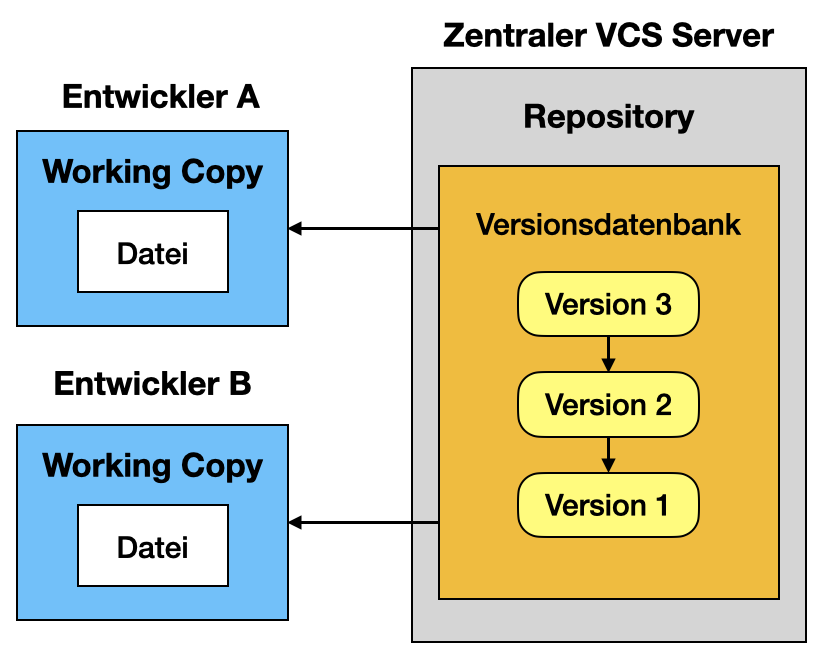
\includegraphics[scale=.65]{images/central_vcs.png}
	\end{center}
		\caption{Zentralisiertes Versionskontrollsystem}
	\end{figure}
	
	\item \textbf{Verteiltes VCS:} Im Gegensatz zum zentralisierten VCS existiert beim verteilten Versionskontrollsystem kein zentrales Repository. Jeder am Projekt tätige Entwickler verfügt über ein eigenes Repository, das er mit anderen Repositories abgleichen kann. Auch hier ist die History klar ersichtlich. Der einzige Unterschied zu 	den beiden anderen Versionskontrollsystemen ist der, dass Änderungen hier am lokalen Rechner erfolgen können. Eine Verbindung mit dem Server ist nicht notwendig.
	
	\begin{figure}[H]
	\begin{center}
		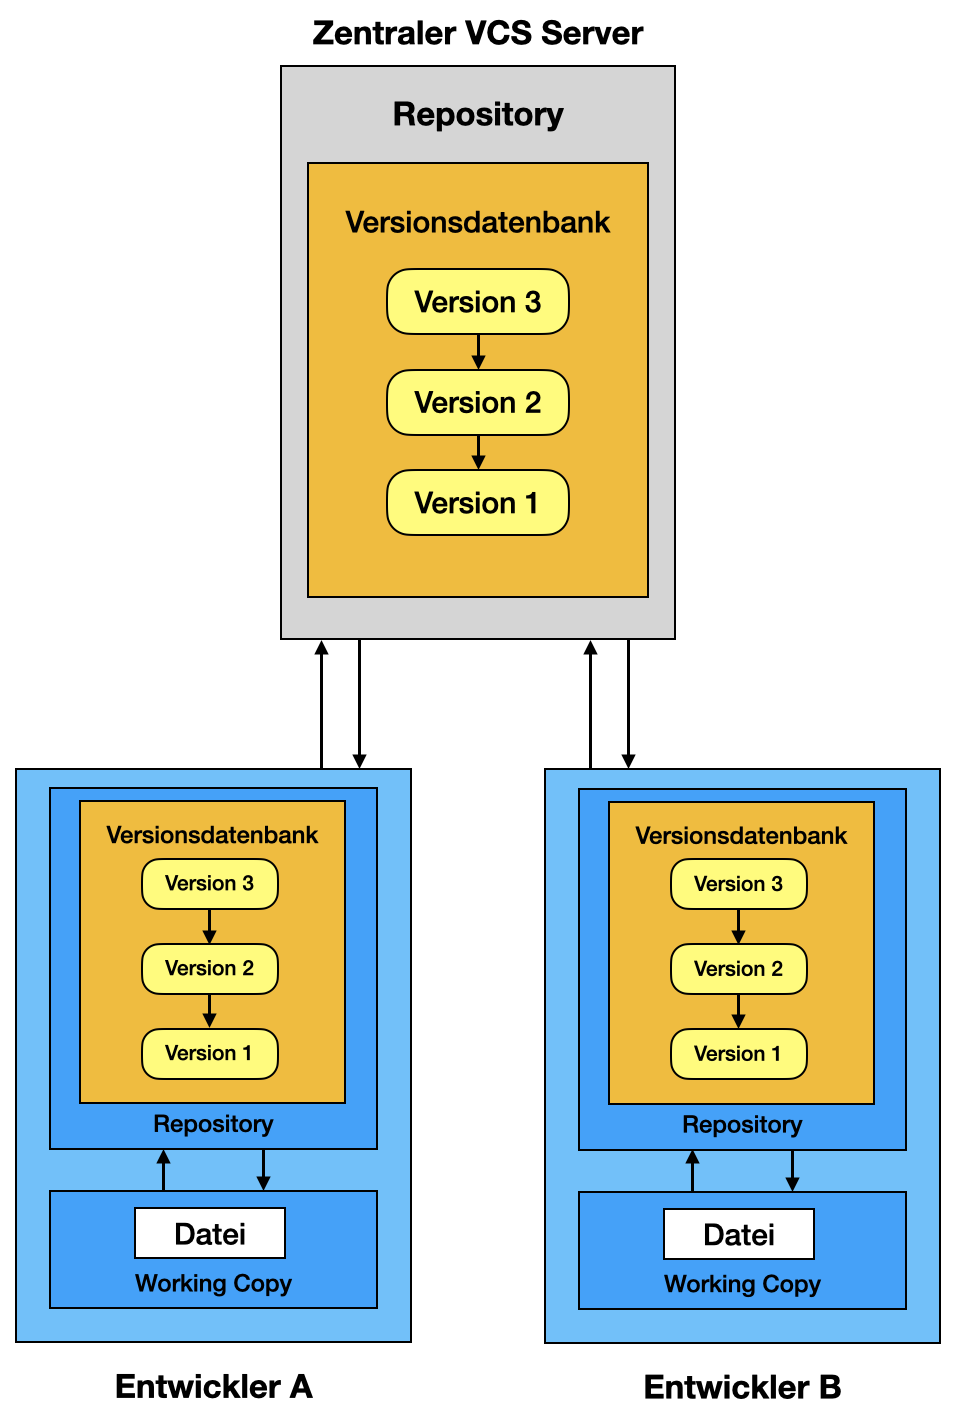
\includegraphics[scale=.6]{images/distributed_vcs.png}
	\end{center}
		\caption{Verteiltes Versionskontrollsystem}
	\end{figure}
\end{itemize}

\subsection{Git}
Git ist ein Open-Source-Tool, das von Linus Torvalds, dem Entwickler des Betriebssystems Linux, entwickelt wurde und stammt aus dem Jahr 2005 (Atlassian, vgl. \cite{atlassian_git_2020}, 15.11.2020). Heutzutage zählt es zu eines der weitverbreitesten Versionsverwaltungssysteme weltweit. Die Softwareentwickler kommen sowohl aus dem kommerziellen als auch aus dem öffentlichen Bereich. Aufgrund seiner Architektur ist Git ein Distributed VCS (DVCS, dt. verteiltes VCS) und funktioniert in zahlreichen Plattformen und Entwicklungsumgebungen. Das bedeutet, dass auf die gesamte History mit allen Entwicklungsarbeiten von jedem Standort aus zugegriffen werden kann. Neben seinem verteilten System ist Git unter anderem auf Performance, Sicherheit und Flexibilität fokussiert.

\paragraph{Snapshots}\mbox{}\\
Bei den meisten VCS werden Informationen als eine Liste mit den Änderungen innerhalb der Dateien gespeichert. Das bedeutet, dass bei jeder Version nur die Dateien festgehalten werden, deren Inhalt sich während den Entwicklungsarbeiten geändert haben.

\begin{figure}[H]
\begin{center}
	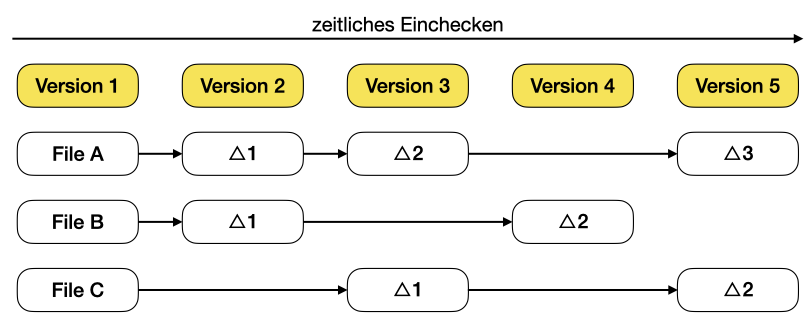
\includegraphics[scale=.4]{images/other_vcs.png}
\end{center}
	\caption{Speichern von Daten bei anderen VCS}
\end{figure} 

\mbox{}\\Im Gegensatz dazu werden die Daten als eine Art Folge von Schnappschüssen (engl. snapshots) betrachtet. Nach jedem Commit wird der aktuelle Stand des Repositories gespeichert. Dieser beinhaltet die gesamte Kopie des Projekts zu diesem Zeitpunkt und erhält eine Referenz zu diesem Schnappschuss in Form eines einzigartigen Hashwertes. Wenn das Entwicklerteam weiter am Projekt arbeitet und die Änderungen committet, erhalten die neuen und geänderten Dateien eine neuen Commit-Hash, während die Dateien, die sich nicht geändert haben, nur auf dieselbe Datei im vorherigen Schnappschuss verlinkt werden.

\begin{figure}[H]
\begin{center}
	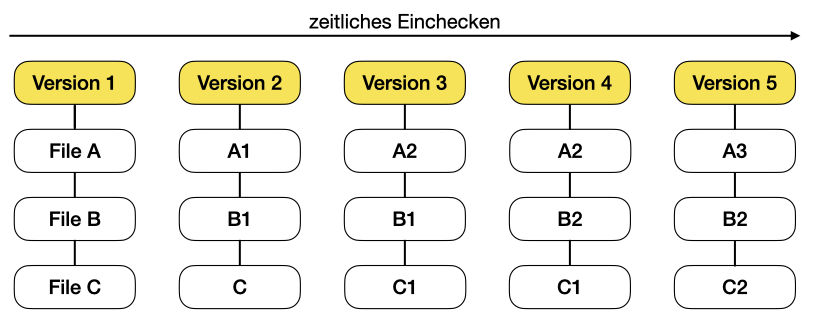
\includegraphics[scale=.4]{images/git_snapshot.png}
\end{center}
	\caption{Speichern von Daten bei Git}
\end{figure}

\mbox{}\\Um eine Sicherheit garantieren zu können, werden die Dateiinhalte sowie ihre Beziehungen zu anderen Dateien, Verzeichnissen, Versionen, Commits und Tags mit dem Hashing-Algorithmus SHA1 gesichert. Dadurch kann der Quellcode des Entwicklers vor ungewollten Änderungen geschützt und die Historie vollständig mitverfolgt werden. In der Datenbank werden keine Dateinamen sondern nur Hashwerte gespeichert. Ein Beispiel für so einen Wert ist \texttt{fe215ed7198155ca796fbb8ef81683137c210492}.\\

\paragraph{Workflow}\mbox{}\\
In einem Git-Projekt sind die drei wichtigsten Stufen das Working Directory, die Staging Area und das Repository, wobei dieses in das \texttt{local} und das  \texttt{remote} Repository gegliedert werden kann. Mit  \texttt{add} wird eine Kopie des Working Directory erstellt, wobei die Änderungen an den Dateien mit  \texttt{new},  \texttt{modified} oder  \texttt{deleted} gekennzeichnet sind. Die Arbeitskopie befindet sich nun in der Staging Area und noch nicht in der Datenbank. Nun haben die Dateien den Status  \texttt{staged} und können im nächsten Schnappschuss eingepflegt werden. Nach einem  \texttt{commit} wird ein Schnappschuss im lokalen Repository erstellt, der mit einem  \texttt{push} in der Datenbank und somit im entfernten Repository gesichert wird.

\begin{figure}[H]
\begin{center}
	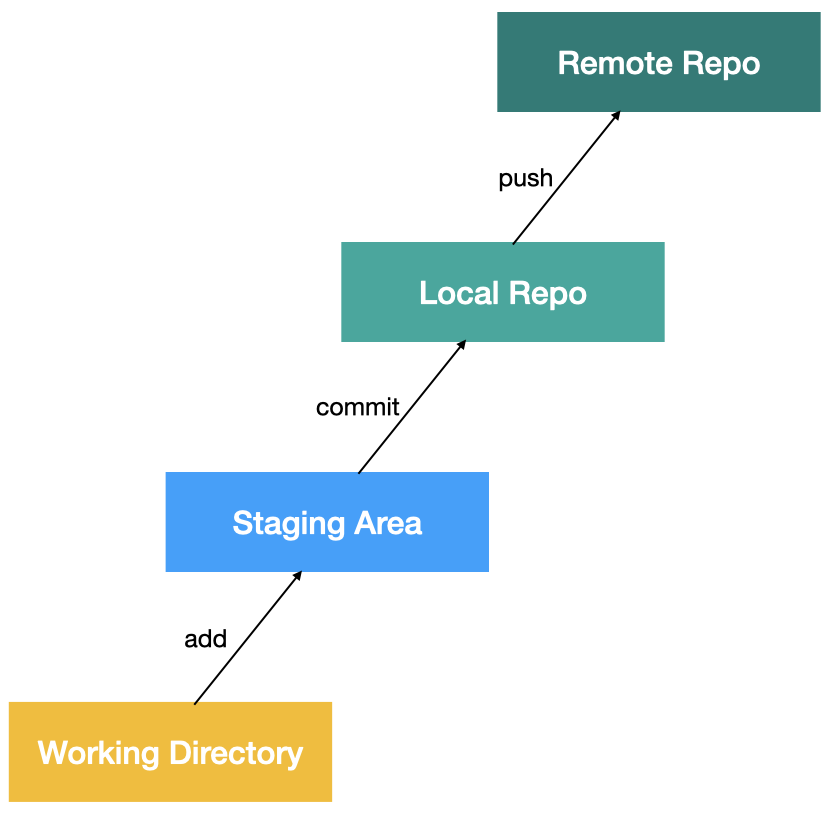
\includegraphics[scale=.3]{images/git_workflow.png}
\end{center}
	\caption{Die drei Hauptstufen von Git}
\end{figure}

\paragraph{Merge}\mbox{}\\
Oftmals werden Entwicklungszweige erstellt um Bugs zu beheben oder an neuen Funktionalitäten einer Software zu arbeiten. Diese Änderungen sollen zu einem späteren Zeitpunkt in einen einzigen Branch integriert werden, der in den meisten Fällen der Hauptzweig \texttt{master} ist. Dies wird durch einen Merge ermöglicht.

 \mbox{}\\
Mehrere Commits aus zwei Entwicklungszweigen werden in einen einheitlichen Verlauf zusammengeführt und die Branches somit vereint. Im Prinzip sucht sich der Pointer der Commits einen gemeinsamen Commit als Basis des Merges. Genau dann, wenn diese Basis gefunden wird, wird ein zusätzlicher Commit für den Merge erstellt. Dadurch werden alle seither vorgenommenen Änderungen in einen gemeinsamen Verlauf vereint.

\begin{figure}[H]
\begin{center}
	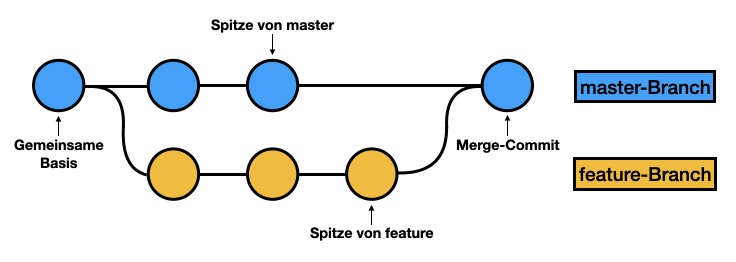
\includegraphics[scale=.8]{images/git-merge.png}
\end{center}
	\caption{Mergen von zwei Branches mit Merge-Commit}
\end{figure}

 \mbox{}\\
Im Gegensatz zu einfachen Commits während der Entwicklung, haben Merge-Commits zwei übergeordnete Commits. Sind Änderungen in beiden Branches vorgenommen worden, können von Git nicht automatisch zusammengeführt werden. Dies führt oftmals zu einem Merge-Konflikt, der von dem Entwickler manuell beseitigt werden muss. Im Normalfall kann Git die Commit-Historie automatischen zusammenführen, es sei denn es gibt Änderungen im aktuellen Branch und im Ziel-Branch, die zu Konflikten im Projekt führen.

 \mbox{}\\
Grundsätzlich gibt es zwei Arten von Merges (Atlassian, vgl. \cite{atlassian_git_merge_2021}, 09.04.2020):

\begin{itemize}
	\item \textbf{Fast-Forward-Merge:}\\
		Wenn der Verlauf vom aktuellen Entwicklungszweig zum Ziel-Branch linear ist, findet ein Fast-Forward-Merge
		statt. Linear bedeutet, dass nur an einem Entwicklungszweig Änderungen vorgenommen worden sind und der 
		andere genauso geblieben ist, wie zu dem Zeitpunkt, an dem der andere Branch erstellt worden ist.\\
		Bei diesem Merge wird ausschließlich der Pointer des Ziel-Branches auf die Commit-Spitze des aktuellen 
		Branches gelegt. Somit werden die beiden Entwicklungszweige kombiniert und enthalten dieselbe 
		Commit-Historie. Da lediglich die Position des Pointers verändert wird, erstellt Git keinen Merge-Commit. 
		Für den Fall, dass kein linearer Pfad zum Ziel-Branch existiert, erfolgt das Zusammenführen der Branches
		mit einem 3-Way-Merge. 
		
		\begin{figure}[H]
		\begin{center}
			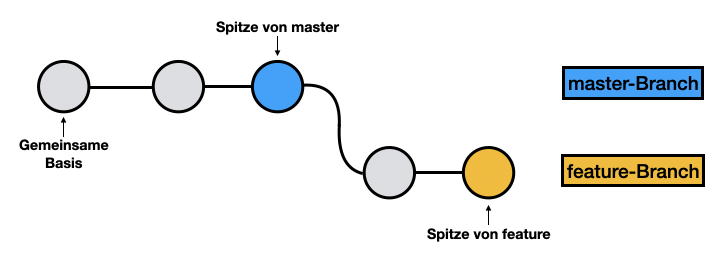
\includegraphics[scale=.8]{images/git-fast-forward-merge-before.png}
		\end{center}
			\caption{Es werden Änderungen am \texttt{feature}-Branch vorgenommen, der \texttt{master}-Branch
				bleibt gleich.}
		\end{figure}
		
		\begin{figure}[H]
		\begin{center}
			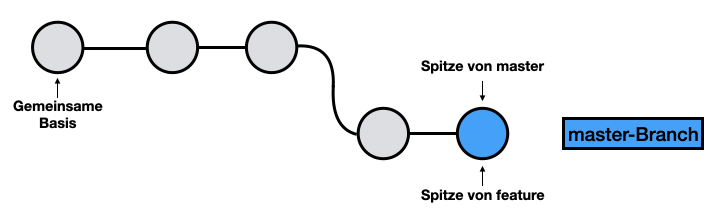
\includegraphics[scale=.8]{images/git-fast-forward-merge-after.png}
		\end{center}
			\caption{Die Änderungen des \texttt{feature}-Branches werden in den \texttt{master}-Branch eingepflegt.}
		\end{figure}
		
	\item \textbf{3-Way-Merge:}\\
		Die Bezeichnung 3-Way-Merge kommt daher, dass für das Zusammenführen von zwei Entwicklungszweigen 
		drei Commits benötigt werden. Zwei Commits sind die Spitzen der beiden Branches und ein Commit ist ihr
		gemeinsamer Basis-Commit.\\
		Hierbei werden seit der Erstellung eines neuen Entwicklungszweiges sowohl 
		am Ziel-Branch als auch am aktuellen Branch neue Änderungen gemacht, die wieder zusammengeführt
		werden sollen. Vor allem beim Entwickeln neuer umfangreicher Funktionalitäten oder beim zeitgleichen 
		Arbeiten am selben Projekt mit mehreren Entwicklern, ist ein 3-Way-Merge erforderlich. \\
		Allerdings kann es hierbei zu Konflikten während eines Merges kommen, die von dem Entwickler selbst
		gelöst werden muss.
		
		\begin{figure}[H]
		\begin{center}
			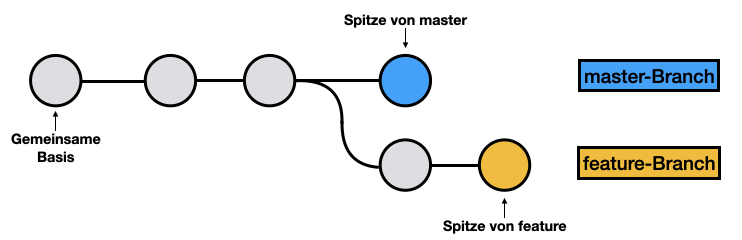
\includegraphics[scale=.8]{images/git-3-way-merge-before.png}
		\end{center}
			\caption{Es werden Änderungen am \texttt{feature}-Branch am \texttt{master}-Branch vorgenommen.}
		\end{figure}
		
		\begin{figure}[H]
		\begin{center}
			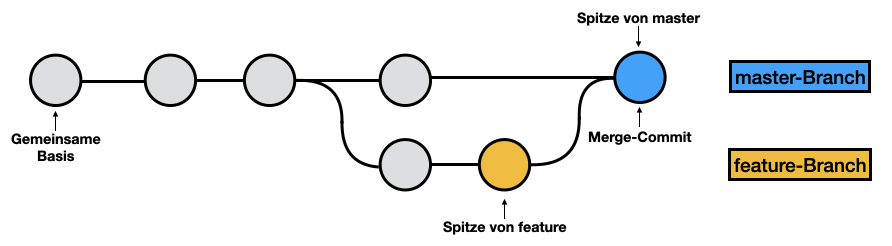
\includegraphics[scale=.8]{images/git-3-way-merge-after.png}
		\end{center}
			\caption{Die Änderungen des \texttt{feature}-Branches werden mit einem Merge-Commit in den 
				\texttt{master}-Branch eingepflegt.}
		\end{figure}
\end{itemize}

\subsection{GitLab}
Im Jahr 2011 ist GitLab von den ukrainischen Entwicklern Dmitri Saparoschez und Valery Sizov ursprünglich in der Programmiersprache Ruby on Rails und mittlerweile noch zusätzlich in Go und Vue.js geschrieben worden. Es ist eine Webapplikation zur Versionskontrolle, das auf Git basiert, in mehr als 100.000 Unternehmen zum Einsatz kommt und von etwa 30 Millionen registrierten Benutzern genutzt wird (GitLab, vgl. \cite{gitlab_2020}, 30.11.2020). Neben dem Arbeiten mit Git stellt diese Anwendung einige weitere Funktionen zur Verfügung. Diese sind beispielsweise eine integrierte und kostenlose Continuous Integration/Delivery (CI/CD), das Issue Tracking, die Wiki-Funktion und vieles mehr. Zusätzlich können Rollen zugewiesen werden, die die Berechtigungen von den jeweiligen Nutzern festlegen.

\mbox{}\\Seit 2013 gibt es zwei Linzenzmodelle von GitLab. Die Community Edition (CE) wird unter der MIT-Lizenz als Open-Source-Software entwickelt und ist auf gitlab.com als Software as a Service (SaaS) erreichbar. Hingegen wird die Enterprise Edition unter einer proprietären Lizenz entwickelt und beinhaltet mehr Funktionen, die für Unternehmen relevanter sind.

\section{Hypertext Markup Language}
Hypertext Markup Language, kurz HTML, ist eine Auszeichnungssprache, welche den Inhalt und die Struktur einer Webseite definiert. Die Strukturierung kann dabei in Paragraphen, Listen, Bildern, Tabellen und einigen anderen Elemente erfolgen (MDN Web Docs, vgl. \cite{html_2021}, 10.04.2021). 

\mbox{}\\
\textbf{''Hypertext''} bezeichnet die Links, die entweder auf HTML-Elemente innerhalb einer Webseite verlinkt oder mehrere Webseiten miteinander verbindet. Grundsätzlich werden mithilfe von Links Inhalte in das Internet hochgeladen und mit Seiten verlinkt.\\
\textbf{''Markup''} dient dazu Texte, Bilder sowie weitere Inhalte zur Darstellung in einem Webbrowser zu annotieren.\\
Ein HTML-Element wird in den sogenannten \textbf{''Tags''} auf einer Webseite platziert. Dabei wird der Name des Elementes zwischen die Klammern \texttt{<} und \texttt{>} gegeben. Diese Tags sind case-insensitive, weshalb sie in Groß- oder Kleinbuchstaben oder in einer Mischung dieser geschrieben werden können. Beispielsweise kann ein \texttt{<label>} Tag auch als \texttt{<LABEL>} oder \texttt{<Label>} definiert werden.

\mbox{}\\
Zusätzlich zu HTML kommen andere Technologien wie Cascading Style Sheets, auch CSS, und JavaScript zum Einsatz. Dabei beschreibt CSS das Aussehen der Webseite während JavaScript die Funktionalität und das Verhalten festlegt. 

\subsection{HTML-Elemente}

\paragraph{Aufbau}

\mbox{}\\
Ein HTML-Element ist vorwiegend zusammengesetzt aus einem öffnenden und einem schließenden Tag sowie der Inhalt zwischen diesen Tags. Es ist eine Art Container oder Behälter für die Informationen, die innerhalb von ihm definiert sind.

\begin{figure}[H]
	\begin{center}
		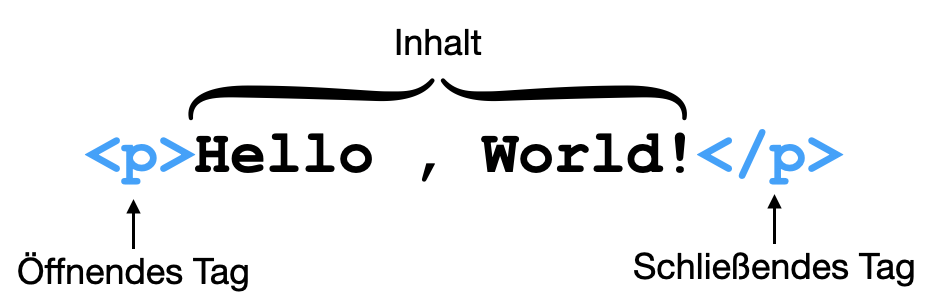
\includegraphics[scale=.6]{images/html-element-example.png}
	\end{center}
		\caption{Beispiel eines HTML-Elementes}
\end{figure}

\begin{itemize}
	\item Das \textbf{öffnende Tag} ist zusammengesetzt aus spitzen Klammern \texttt{< >}, die den Namen des 
		HTML-Elementes 
		umschließen. Es gibt die Stelle an, an der das Element beginnt.
	\item Das \textbf{schließende Tag} ist ähnlich dem öffnenden Tag nur, dass zusätzlich ein Schrägstrich \texttt{/} vor dem
		Namen des HTML-Elementes steht. Es gibt die Stelle an, an der das Element endet. 
	\item Der \textbf{Inhalt} des HTML-Elementes steht zwischen diesen beiden Tags. In der Abbildung handelt es sich hierbei 
		um einen simplen Text.
\end{itemize}

\mbox{}\\
Des Weiteren können HTML-Elemente Attribute beinhalten, die in den spitzen Klammern und nach dem Namen des öffnenden Tags geschrieben werden. Attribute geben Auskunft über zusätzliche Informationen über das Element, der nicht im Inhalt ersichtlich sein soll. Dabei müssen folgende Voraussetzungen erfüllt sein:

\begin{itemize}
	\item Zwischen dem HTML-Elementname und dem Attribut oder mehreren Attributen muss ein Leerzeichen sein.
	\item Nach dem Attributnamen folgt ein Gleichheitszeichen \texttt{=}.
	\item Der Attributwert muss von Anführungszeichen \texttt{"} umschlossen sein.
\end{itemize}

\paragraph{Verschachtelte Elemente}
\mbox{}\\
HTML-Elemente, die sich innerhalb eines Elementes befinden, werden als Verschachtelung bezeichnet. Dabei muss stets darauf geachtet werden, dass die Tags wieder korrekt geschlossen werden. Befindet sich zum Beispiel ein \texttt{<strong>} Tag innerhalb eines \texttt{<p>} Tag, muss darauf geachtet werden, dass der innere Tag vor dem äußeren Tag geschlossen wird. 

\paragraph{Leere Elemente}
\mbox{}\\
Obwohl die meisten HTML-Elemente einen Inhalt haben, gibt es dennoch einige, die keinen besitzen. Dazu zählt beispielsweise der \texttt{<img>} Tag. Bei diesem Element gibt es keinen schließenden Tag und es umhüllt auch keinen Inhalt. Der Zweck hinter
diesen Tags ist es, einzelne Gestaltungselemente einzubinden.

\begin{figure}[H]
	\begin{center}
		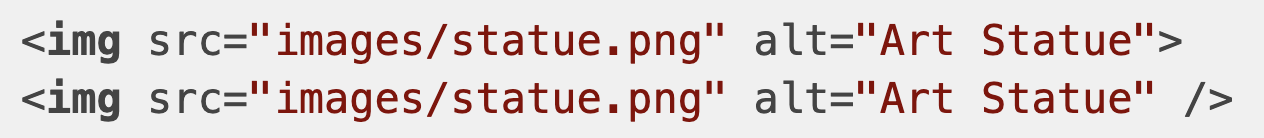
\includegraphics[scale=.5]{images/empty-element-example.png}
	\end{center}
		\caption{Beispiel von zwei leeren HTML-Elementen ohne und mit geschlossenem Ende}
\end{figure}

\mbox{}\\
Damals ist mit Extensible HTML, kurz XHTML am Ende eines leeren HTML-Tags ein Schrägstrich gesetzt worden. Mit HTML5 kann dieser weggelassen werden. 

\subsection{Aufbau eines HTML-Dokumentes}

\begin{figure}[H]
	\begin{center}
		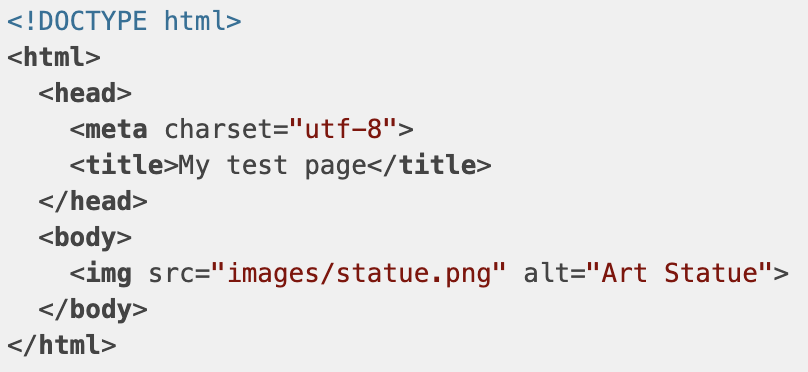
\includegraphics[scale=.7]{images/html-document-structure.png}
	\end{center}
		\caption{Aufbau eines HTML-Dokumentes}
\end{figure}

Die folgenden HTML-Tags bilden zusammen eine HTML-Seite:

\begin{table}[H]
	\begin{center}
	\begin{tabular}{| c | m{10cm} |}
		\hline
 		\cellcolor{Gray}\textcolor{White}{HTML-Element} & \cellcolor{Gray}\textcolor{White}{Beschreibung}  \\
		\hline
		\texttt{<!DOCTYPE html>} & Früher hat dieses Tag dazu gedient, um mit Prüfung von Fehlern und anderen 
			Überprüfungen sicherzustellen, dass die HTML-Seite gut dargestellt wird und funktioniert. Heute dient dieses Tag 
			lediglich dazu, um sicherzugehen, dass das Verhalten des Dokumentes korrekt ist.\\
		\hline
		\texttt{<html></html>} & Diese Element schließt den gesamten Inhalt einer HTML-Seite ein und wird auch als Root-
			Element bezeichnet.\\
		\hline
		\texttt{<head></head>} & Dieses Element ist eine Art Container und umfasst alles, was auf der Webseite beinhaltet, 
			aber nicht für den Betrachter sichtbar sein soll. Dazu zählen zum Beispiel Gestaltungen mit CSS, 
			Zeichensatzdeklarationen und vieles mehr.\\
		\hline
		\texttt{<title></title>} & Damit wird der Titel der Webseite beschrieben, der in der Registerkarte des Browsers angezeigt 
			wird.\\
		\hline
		\texttt{<body></body>} & Dieser HTML-Tag beinhaltet den Inhalt, der für die Benutzer der Webseite angezeigt wird. \\
		\hline
	\end{tabular}
	\end{center}
	\caption{Unterstützte Funktionalitäten der Tastatur}
\end{table}

\newpage
\section{JavaScript}
JavaScript, kurz JS, basiert auf dem ECMAScript Standard und ist eine dynamische, funktionale und objektorientierte Skriptsprache, die im Mai 1995 innerhalb von 10 Tagen von Brendan Eich entwickelt worden ist (MDN Web Docs, vgl. \cite{javascript_2021}, 11.02.2021). Erstmals ist sie bei Netscape für dynamisches HTML in Webbrowsern zum Einsatz gekommen. Mittlerweile wird JS auch auf Servern oder Mikrocontrollern verwendet.

\subsection{ECMAScript}
ECMAScript ist von Brendan Eich bei Netscape entwickelt worden und gibt vor welche JavaScript Funktionalitäten von Webbrowsern implementiert werden müssen (Harband und Smith 2020, vgl. \cite{ecma_2020}, 10.04.2021). Somit kann erreicht werden, dass Webseiten ohne Bedenken in jedem beliebigen Browser funktionsfähig sind. Gäbe es diesen Standard nicht, müssten Polyfills eingesetzt werden. Diese würden Funktionalitäten in JavaScript implementieren, die jeder Browser verstehen sollte. Diese Notlösung führt dazu, dass zusätzlich mehr programmiert wird, der Nutzer viel größere Dateien herunterladet, die Lösung nicht nativ ist und die Performance darunter leidet. 

\subsection{Dynamische Typisierung}
JavaScript ist schwach typisierte und dynamische Programmiersprache. Wenn Variablen erstellt werden, haben sie keinen expliziten Datentyp. Anhand des Wertes einer Variable ändert sich intern auch ihr Datentyp. Der aktuellste ECMAScript Standard definiert neun Typen, die in zwei Kategorien unterteilt werden können.

\paragraph{Primitive Datentypen:}

\begin{itemize}
	\item \texttt{undefined}: Die Variable hat keinen Datentyp oder wurde explizit als \texttt{undefined} angegeben.
	\item \texttt{Boolean} ist ein logischer Datentyp der einen Wahrheitswert  \texttt{true} oder  \texttt{false} annehmen 	
		kann.
	\item \texttt{Number} ist ein numerischer Datentyp, der dem IEEE 754 konform ist. Das heißt, dass fast alle Zahlen, 
		inklusive ganze Zahlen als Gleitkommazahl gespeichert werden.
	\item \texttt{String} ist eine Sequenz von Buchstaben.
	\item \texttt{BigInt} ist ein numerischer Datentyp, der ganze Zahlen in der Langzahlarithmetik darstellt.
	\item \texttt{Symbol} ist ein eindeutiger String, der nicht mehrmals erstellt werden kann. Es wird als Objekteigenschaft 
		verwendet. Somit können JavaScript-Objekte wiederholt denselben Eigenschaftsnamen verwenden.
	\item \texttt{null} gibt an, das absichtlich ein Wert fehlt und die Variable auf kein Objekt zeigt.
\end{itemize}

\paragraph{Strukturierte Typen:}

\begin{itemize}
	\item \texttt{Object}: Alle Variablen, die mit  \texttt{new} angelegt werden, sind Objekte. Dazu zählt auch das 
		JavaScript-Objekt \texttt{\{ ... \}}.
	\item \texttt{Function} gibt den Datentypen an, die als JavaScript-Funktion mit dem Schlüssenwort \texttt{function}
		deklariert worden ist.
\end{itemize}

\paragraph{Unterschied zwischen \texttt{==} und \texttt{===}}

\mbox{}\\
\texttt{==} überprüft auf Gleichheit der beiden Variablen. Sollten diese nicht vom gleichen Typ sein, werden diese auf denselben Datentyp konvertiert. Referenzen gelten gleich, wenn sie auf dasselbe Objekt zeigen.

\begin{itemize}
	\item \texttt{1 == 1}
	\item \texttt{'1'== 1}
	\item \texttt{1 == true}
	\item \texttt{0 == false}
\end{itemize}

\mbox{}\\
\texttt{===} achtet genauso wie oben genannt auf den Inhalt mit dem Unterschied, dass davor überprüft wird, ob beide Variablen denselben Typ haben.

\mbox{}\\
Dasselbe gilt für die Überprüfung der Ungleichheit \texttt{!=} und \texttt{!==}.

\section{TypeScript}
TypeScript (TS) ist eine Erweiterung von JavaScript und basiert ebenfalls auf den ECMAScript Standards (Malcher, Hoppe und Koppenhagen 2020, vgl. \cite{typescript_2020}). Im Gegensatz zu JavaScript besitzt TypeScript ein statisches Typsystem. An und für sich wird TypeScript nicht von Browsern unterstützt, denn es handelt sich um eine Programmiersprache, die mittels eines Kompilierers diese Sprache auf JavaScript umwandelt. Man spricht hierbei von einem Transpiler. Mit einem Typsystem ist es möglich, bereits zur Entwicklungszeit Fehler und Probleme ausfindig zu machen.\\
TypeScript ermöglicht auch die Verwendung von neuen ECMAScript-Features, weshalb Projekte mit den neuesten Features erstellt werden können. Der Kompilierer ist dafür zuständig, das Browser mit älteren Versionen des ECMAScriptes den transpilierten Code ausführen können.

\newpage
\subsection{Typen}
Wie zuvor erwähnt worden ist, ist eine der Stärken von TypeScript die Typisierung. Es werden einige primitive Datentypen mitgeliefert. Zu denen gehören \texttt{number}, \texttt{string} und \texttt{boolean}.

\begin{itemize}
	\item \texttt{number} umfasst alle Gleitkommazahlen sowie ganze Zahlen.
	\item \texttt{string} definiert eine Zeichenkette.
	\item \texttt{boolean} kann die Wahrheitswerte \texttt{true} oder \texttt{false} annehmen.
\end{itemize}

\mbox{}\\
Variablen, die mit diesen jeweiligen Typen definiert sind, dürfen keinen anderen Wert annehmen, der nicht ihrem Datentyp entspricht. Ansonsten wird ein Fehler vom Kompilierer geworfen. Einige Entwicklungsumgebung besitzen ebenfalls die Funktion diese Fehler erkennen zu können.

\begin{figure}[H]
	\begin{center}
		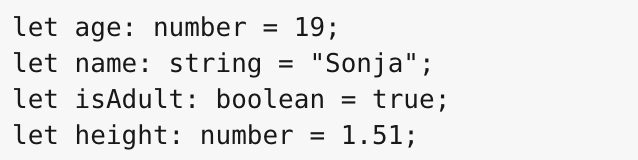
\includegraphics[scale=.7]{images/typescript-primitve-types.png}
	\end{center}
		\caption{Variablen mit primitiven Datentypen}
\end{figure}

\mbox{}\\
Neben den primitiven Datentypen gibt es die beliebigen Werte \texttt{any} und \texttt{unknown}. Diese Datentypen sind dynamisch und können jeden möglichen Wert annehmen, ohne dass sich der Kompilierer beschwert. 

\subsection{Union Types}
Union Types beschreiben Typen, die aus mehren Typen zusammengesetzt sind. Ein geeignetes Beispiel hierfür ist die Hausnummer. Sie kann entweder eine Zahl oder eine Zahl mit Buchstaben sein.

\begin{figure}[H]
	\begin{center}
		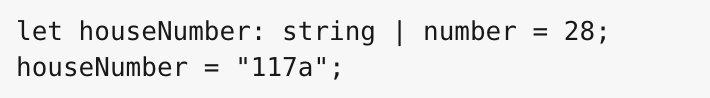
\includegraphics[scale=.7]{images/typescript-union-types.png}
	\end{center}
		\caption{Variable mit mehreren Typen}
\end{figure}

\subsection{Type Definition}
Angenommen es gibt eine JavaScript Bibliothek, die oft zum Einsatz kommt und unter anderem wird diese auch für TypeScript Projekte verwendet. Allerdings kann TypeScript nichts mit dieser Bibliothek anfangen, da die Typen nicht existent sind. Genau aus diesem Grund werden Type Definitions verwendet. Sie werden mit den jeweiligen JavaScript-Dateien geliefert und beinhalten keinen Quellcode, sondern lediglich nur Informationen zu diesem. Dazu gehören Informationen wie Datentypen, Konstanten und Funktionen mit Parameter- und Rückgabetypen.

\mbox{}\\
Eine Funktion wird vom TypeScript-Compiler in JavaScript umgewandelt und verliert somit jegliche Informationen zu den vorher festgelegten Datentypen. Daher können Dateien für Type Definitions generiert oder erstellt werden.

\begin{figure}[H]
	\begin{center}
		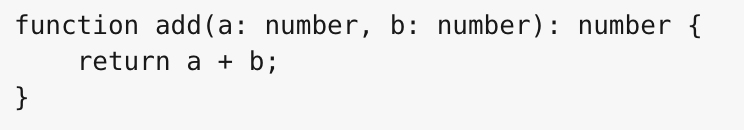
\includegraphics[scale=.7]{images/typescript-type-definition-1.png}
	\end{center}
		\caption{Funktion zum Addieren von zwei Zahlen in TypeScript}
\end{figure}

\begin{figure}[H]
	\begin{center}
		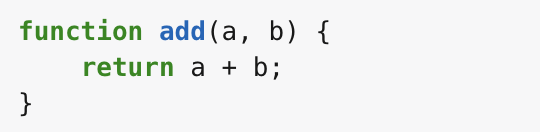
\includegraphics[scale=.7]{images/typescript-type-definition-2.png}
	\end{center}
		\caption{Funktion zum Addieren von zwei Zahlen in JavaScript}
\end{figure}

\begin{figure}[H]
	\begin{center}
		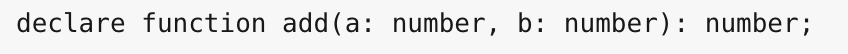
\includegraphics[scale=.7]{images/typescript-type-definition-3.png}
	\end{center}
		\caption{Type Definition für die Funktion zum Addieren von zwei Zahlen}
\end{figure}

\subsection{TypeScript Compiler}
Der TypeScript Compiler gibt dem Entwickler einen Spielraum, gewisse Einstellungen zu definieren. Dazu zählen strikte Null-Überprüfungen, wo ein Fehler geworfen wird, wenn die Variable \texttt{null} sein kann und nicht überprüft wird. Außerdem kann der Datentyp \texttt{any} ausgeschaltet werden für eine genauere Datentypisierung. Variablen, die nicht verwendet werden, wie beispielsweise lokale Variablen oder Parametervariablen, können so eingestellt werden, dass ein Fehler geworfen wird. Für eine einfachere und angenehmere Entwicklung können Source-Maps aktiviert werden. Diese dienen zur Anzeige des Quellcodes in TypeScript, wenn Fehler im Browser geworfen werden oder ein Debug durchgeführt wird.

\section{Node.js und npm}

\subsection{Node.js}
Node.js ist eine JavaScript-Laufzeitumgebung mit der JavaScript-Code außerhalb eines Webbrowsers ausgeführt werden kann (OpenJS Foundation, vgl.\cite{nodejs_2021}, 10.04.2021). Somit kann der Code nicht nur clientseitig, sondern auch serverseitig verwendet werden. Node.js hat eine eventbasierte Architektur und wird auf der im Jahr 2009 von Google entwickelten Open-Source-JavaScript-Engine V8 ausgeführt, der ursprünglich nur für Browser verwendet worden ist.\\
Zu den Einsatzgebieten gehören die Entwicklung von Webservern, die Erstellung von Skripten oder Tools im Terminal sowie seit neuestem die Entwicklung von Desktopanwendungen. Neben der Laufzeitumgebung stellt Node.js seine Core-API zur Verfügung. Diese reicht von simplen Netzwerkzugriffen bis hin zu Zugriffen auf Dateien.

\paragraph{Vorteile und Gründe zur Verwendung von Node.js}
\mbox{}\\
Mit seiner eventbasierten Architektur führt Node.js nur einen einzigen Thread aus, in dem ein Event Loop läuft. Im Gegensatz zu Node.js verwenden traditionelle Webframeworks für jede Anfrage auf den Server einen eigenen Thread. Näher betrachtet kann das Starten eines Threads einige Nachteile mit sich bringen. Angenommen ein Thread, der lediglich die Anfrage bearbeitet, benötigt 2 MB im Hauptspeicher, beginnt die Überlastung eines Servers mit 8 GB Hauptspeicher und 4000 gleichzeitigen Anfragen. Ein weiteres Beispiel ist in Blogpost von caustik's blog zu finden (caustik's blog 2012, vgl. \cite{nodejs_blogpost_2012}, 13.02.2021).\\
Mit der Verwendung eines einzigen Threads, muss auch dementsprechend mit Gefahren gerechnet werden.

\mbox{}\\
Rechenintensive Anfragen könnten den einzigen Thread überlasten und alle anderen Anfragen verzögern. Diese Verlangsamung würde solange andauern bis dieser rechenintensive Prozess fertig ausgeführt worden ist. Im Normalfall wird bei einer Exception oder bei einem Fehler der Thread gestoppt. Ist allerdings nur ein einzelner Thread vorhanden, kann ein Fehler bereits zum Absturz des Programmes führen. Um das Abstürzen aufgrund von Exceptions zu vermeiden können diese Fehler mit Callbacks verarbeitet werden.

\paragraph{Konkurrenz}
\mbox{}\\
Deno ist genauso wie Node.js eine JavaScript-Laufzeitumgebung und ist von demselben Entwickler Ryan Dahl (Deno, vgl. \cite{deno_2021}, 13.02.2021). Node.js hat viele Probleme gehabt und die Benutzerfreundlichkeit ist ebenfalls nicht zufriedenstellend gewesen. Aus diesem Grund ist Deno erstmals im Jahr 2018 veröffentlicht worden. Neben JavaScript wird auch TypeScript nativ unterstützt und ein großer Wert auf die Sicherheit mit Erlaubnissen gelegt. Ein Modulsystem wie npm kommt nicht mehr zum Einsatz. Externe Module beziehungsweise Bibliotheken werden mit absoluten Adressen importiert. Dieses Konzept ist von Golang inspiriert.

\subsection{npm}
Node Package Manager, kurz npm, ist ein Paketmanager, der die Verwaltung und Bereitstellung der Module und Abhängigkeiten pflegt (vgl. \cite{npm_2021}, 12.02.2021). Diese und jegliche andere Informationen stehen in der \texttt{package.json} Datei. npm setzt sich aus zwei Komponenten zusammen:

\paragraph{Registry}
\mbox{}\\
Die Registry beziehungsweise das Repository ist eine Plattform von npm selber, welche Entwickler die Möglichkeit gibt, Open-Source Software zu veröffentlichen, die als Packages bekannt sind (vgl. \cite{npm_registry_2021}, 09.04.2021). Der Schwerpunkt liegt hier bei JavaScript Libraries und Frameworks. Außerdem dürfen auch andere Dateien, wie zum Beispiel CSS oder TypeScript Deklarationen, hochgeladen werden.
\\
Für Unternehmen oder Personen, die ihren Code nicht veröffentlichen wollen, besteht die Option sich einer npm Mitgliedschaft anzuschließen. Mit der Mitgliedschaft dürfen die Benutzer private packages hochladen. Die Zugriffsverteilung ist je nach Abonnement unterschiedlich und auf Einzelpersonen oder Mitglieder und Teams eines Unternehmens eingeschränkt.

\mbox{}\\
\textbf{Alternativen für die npm Registry sind:}

\mbox{}\\
\textbf{Verdaccio} ist eine simple und leichtgewichtige Registry zum selber Hosten. Die Open-Source Software eignet sich gut für Personen die sich kaum mit dem Einrichten von Produkten auseinandergesetzt haben, da keine Konfigurationen erforderlich sind (vgl. \cite{verdaccio_2021}, 09.04.2021).

\mbox{}\\
\textbf{Jfrog Artifactory} ist eine sogenannte One-Stop Solution Software. Jfrog Artifactory hat nicht nur die npm Registry integriert, sondern auch andere wie Maven, Rubygems, Docker, Go und etliche andere. Sie wird als die perfekte Lösung für große Unternehmen, die sich mit verschiedenen Technologien beschäftigen, bezeichnet (JFrog Ltd., vgl. \cite{jfrog_2021}, 09.04.2021). Die Zugriffe auf Packages oder zahlreiche andere Repository-Formate erfolgt mit einer Benutzer- und Rechteverwaltung. Jfrog Artifactory kann selbst gehostet oder auf der Cloud von Jfrog bereitgestellt werden.

\paragraph{npm CLI}
\mbox{}\\
Die größte Eigenschaft von der CLI, ist die Installation von einer npm Registry. Als Standard wird die Registry von npm herangezogen. Mit \texttt{npm config set registry https://my-registry.com} kann die Registry geändert werden. Um Abhängigkeiten oder Module zu installieren, wird der Befehl \texttt{npm install my-package} verwendet. Die installierten Packages kommen in den Ordner \texttt{/node\_modules} und werden auch automatisch in die \texttt{package.json} eingepflegt. Somit muss der Entwickler diese Aufgabe nicht händisch übernehmen. Des Weiteren können Packages global installiert werden. Die am weitesten verbreitete Anwendungsfälle sind CLIs die in JavaScript programmiert worden sind. Ein Beispiel dafür wäre das beliebte Web-Framework Angular mit seiner Angular-CLI. Nach der globalen Installation kann man auf das CLI-Programm \texttt{ng} direkt vom Terminal aus zugreifen.\\
Für das Erstellen von npm Projekten wird der Befehl \texttt{npm init} benötigt. Hier fragt die npm CLI nach Informationen wie Projektname, Beschreibung, Author etc.

\section{Jest}
Jest ist ein Testing Framework für die JavaScript-Laufzeitumgebung NodeJS (Facebook, vgl. \cite{jest_2021}, 11.04.2021). Da Jest zuerst die Tests durchführt, die beim letzten Mal fehlgeschlagen sind und anschließend die Tests durchführt, die mehr Zeit beanspruchen, ist das parallele Testen sehr schnell. Jest bietet dem Entwickler die Möglichkeit, die Test Coverage zu evaluieren. Mit der Mocking API kann jedes beliebige Objekt gemockt werden.

\section{Webpack}
Webpack ist ein statischer Modul-Bundler für JavaScript-Applikationen (vgl. \cite{webpack_2021}, 11.02.2021). Mehrere JavaScript-Dateien werden zur Nutzung in einem Webbrowser zusammengeführt und zu einer oder mehreren Dateien gebündelt, abhängig von der Anzahl an Modulen. Diese Module werden intern in einem Abhängigkeitsgraphen dargestellt. Rekursiv beginnt dieser vom Eingangspunkt und fügt alle Abhängigkeiten in diesen Graphen ein. Somit wird nur der Code zusammengebündelt, der auch benötigt wird. \\
Der Vorteil besteht darin, dass schnell eine Datei heruntergeladen werden kann, die verkleinert und gebündelt ist. 

\mbox{}\\
Das Konzept von Webpack kann in sechs Kernpunkte unterteilt werden:

\subsection{Entry}
Der Eingangspunkt gibt an wo Webpack beginnen soll das Bundle zusammenzusetzen. Anhand dieses Punktes kann herausgefunden werden welche Abhängigkeiten direkt oder indirekt benötigt werden, die anschließend in den Abhängigkeitsgraphen eingefügt werden. 

\begin{figure}[H]
	\begin{center}
		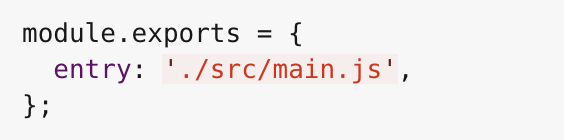
\includegraphics[scale=.7]{images/webpack-entry-point.png}
	\end{center}
		\caption{webpack.config.js}
\end{figure}

\subsection{Output}
Der Output definiert wie Webpack die zusammengebündelten benennen oder wo sie gespeichert werden sollen. 

\begin{figure}[H]
	\begin{center}
		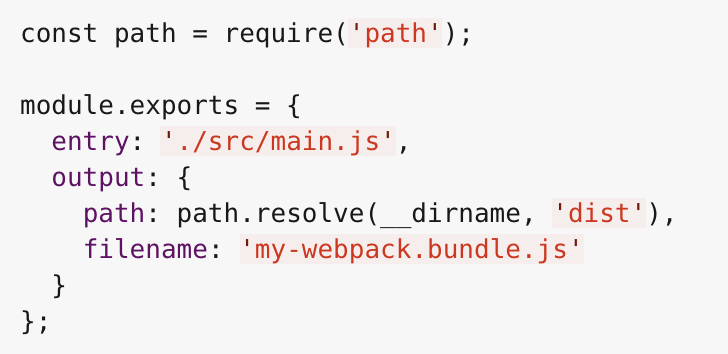
\includegraphics[scale=.7]{images/webpack-output.png}
	\end{center}
		\caption{webpack.config.js}
\end{figure}

\subsection{Loaders}
Webpack unterstützt nur JavaScript und JSON Dateien als Import im Code. Mit Loadern is es möglich Webpack so zu erweitern, dass andere Dateien ebenfalls importiert und in den Abhängigkeitsgraphen eingefügt werden können. Diese Loader besitzen zwei wichtige Eigenschaften:

\begin{enumerate}
	\item \texttt{test} gibt an welche Dateien von diesem Loader verwendet werden. Hierbei handelt es sich um einen 
		regulären Ausdruck.
	\item \texttt{use} legt fest welcher Loader beziehungsweise welche Bibliothek für die Dateien verwendet werden sollen.
\end{enumerate}

\begin{figure}[H]
	\begin{center}
		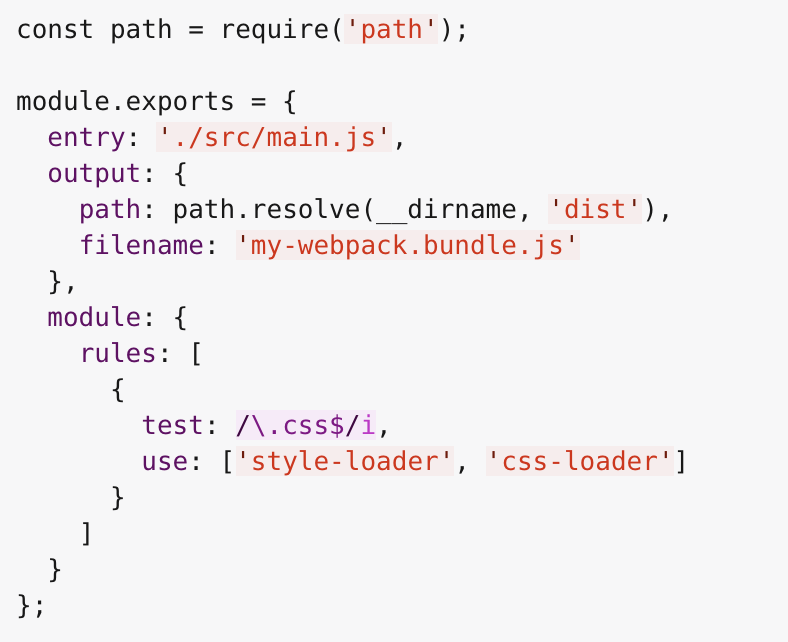
\includegraphics[scale=.7]{images/webpack-loaders.png}
	\end{center}
		\caption{webpack.config.js}
\end{figure}

\mbox{}\\
In der obigen Abbildung ist die Eigenschaft \texttt{rules} definiert mit den beiden erforderlichen Eigenschaften \texttt{test} und \texttt{use}. \texttt{rules} sagt dem Webpack Compiler, dass dieser die Dateien mit der Endung \texttt{.css} innerhalb eines \texttt{require()} oder \texttt{import} Statements mit einem \texttt{css-loader} umwandeln soll. Anschließend werden die transformierten Dateien zum Bundle hinzugefügt.

\subsection{Plugins}
Mithilfe von Plugins besteht die Möglichkeit Webpack so zu erweitern, dass gewisse Funktionalitäten optimiert, automatisiert oder neu hinzugefügt werden. Die Verwaltung von Assets und das Injizieren von Umgebungsvariablen ist ebenso möglich. 
\mbox{}\\
Plugins können verwendet werden, indem das \texttt{require()} Statement verwendet und zum \texttt{plugins}-Array hinzugefügt wird. Mittels Optionen können diese angepasst werden. Ein Plugin kann mehrmals in einer Konfiguration definiert werden, weshalb mit dem \texttt{new}-Operator eine Instanz erstellt werden muss.

\begin{figure}[H]
	\begin{center}
		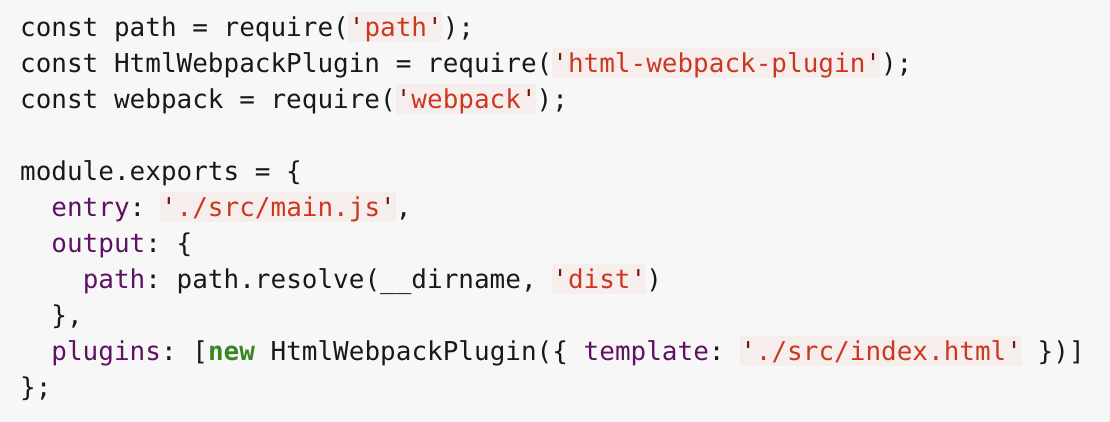
\includegraphics[scale=.7]{images/webpack-plugins.png}
	\end{center}
		\caption{webpack.config.js}
\end{figure}

\mbox{}\\
In diesem Beispiel wird das \texttt{html-webpack-plugin} verwendet, um anhand einer selbstgeschriebenen HTML-Vorlage ein Dokument zu generieren, das die JavaScript und Asset Bundles bereits importiert beziehungsweise referenziert und schließlich  im Output-Ordner \texttt{dist} ablegt.

\subsection{Mode}
Webpack gibt die Möglichkeit zu definieren in welcher Umgebung das Bundle laufen wird. Hierbei können drei verschiedene Modi gesetzt werden: \texttt{development}, \texttt{production} oder \texttt{none}. Dabei versucht Webpack intern, je nach Modus, die bestmögliche Bundle-Optimierung einzusetzen.

\begin{figure}[H]
	\begin{center}
		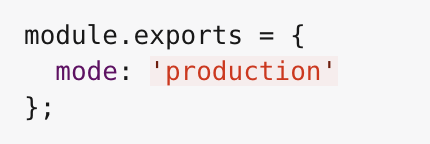
\includegraphics[scale=.7]{images/webpack-mode.png}
	\end{center}
		\caption{webpack.config.js}
\end{figure}

\newpage
\subsection{Browserkompatibilität}
Es ist wichtig zu wissen, dass Webpack alle Browser unterstützt, die ES5-konform sind. Dazu zählen alle moderne und mobile Browser. Ein nichtkompatibler Webbrowser ist beispielsweise der Internet Explorer der Version 8 oder darunter. Falls diese Browser jedoch unterstützt werden sollen, wird ein Polyfill für den JavaScript Standard ES5 benötigt.










